\changecolours{ScoutNavy}
\section{Estruturas Nativas e Modernização com Inteligência Artificial}

% ------------------------------------------------------------------------------
\begin{frame}{As 5 Estruturas de Dados Nativas do Redis}
  \centering
  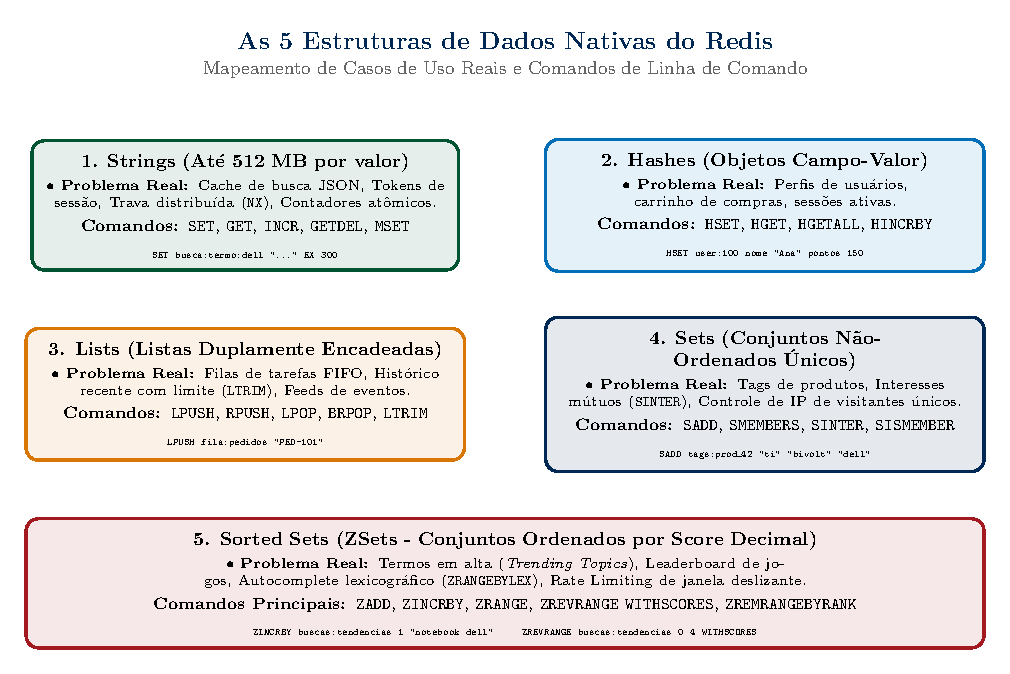
\includegraphics[width=0.90\textwidth,height=0.74\textheight,keepaspectratio]{figuras/fig_estruturas_redis.pdf}
\end{frame}

% ------------------------------------------------------------------------------
\begin{frame}[fragile]{Estrutura 2: Hashes (Objetos Campo-Valor)}
  \begin{columns}[T]
    \begin{column}{0.48\textwidth}
      \alert{Modelagem de Entidades}\par
      \itemseps[topsepi=1mm,itemsepi=1.5mm,labelsep=2mm,leftmargini=4mm]
      \small
      \begin{itemize}
        \item Mapeia dicionários campo-valor sob uma única chave.
        \item Permite alterar campos isolados sem trafegar o JSON todo.
        \item \textbf{Casos Reais:} Perfis de usuários, carrinhos e preferências.
      \end{itemize}
    \end{column}
    \begin{column}{0.50\textwidth}
      \alert{Comandos no redis-cli}\par
      \begin{lstlisting}[language=bash]
# Criar perfil de aluno com campos:
127.0.0.1:6379> HSET user:aluno:42 nome "Ana" pontos 80
(integer) 2

# Incrementar pontuacao atomicamente:
127.0.0.1:6379> HINCRBY user:aluno:42 pontos 20
(integer) 100

# Ler campo isolado em O(1):
127.0.0.1:6379> HGET user:aluno:42 pontos
"100"

# Recuperar todos os pares:
127.0.0.1:6379> HGETALL user:aluno:42
1) "nome"    2) "Ana"
3) "pontos"  4) "100"
      \end{lstlisting}
    \end{column}
  \end{columns}
\end{frame}

% ------------------------------------------------------------------------------
\begin{frame}[fragile]{Estrutura 3: Lists (Filas FIFO e Históricos)}
  \begin{columns}[T]
    \begin{column}{0.48\textwidth}
      \alert{Listas Duplamente Encadeadas}\par
      \itemseps[topsepi=1mm,itemsepi=1.5mm,labelsep=2mm,leftmargini=4mm]
      \small
      \begin{itemize}
        \item Inserção rápida nas pontas (\texttt{LPUSH} / \texttt{RPUSH}).
        \item \textbf{Capped Lists:} \texttt{LTRIM} mantém tamanho fixo.
        \item \textbf{Casos Reais:} Filas de tarefas FIFO e histórico de buscas recentes.
      \end{itemize}
    \end{column}
    \begin{column}{0.50\textwidth}
      \alert{Comandos no redis-cli}\par
      \begin{lstlisting}[language=bash]
# Adicionar buscas recentes:
127.0.0.1:6379> LPUSH hist:42 "python" "nosql" "redis"
(integer) 3

# Manter apenas as 2 mais recentes:
127.0.0.1:6379> LTRIM hist:42 0 1
OK

# Consultar historico podado:
127.0.0.1:6379> LRANGE hist:42 0 -1
1) "redis"  2) "nosql"

# Consumir da ponta oposta (FIFO):
127.0.0.1:6379> RPOP hist:42
"nosql"
      \end{lstlisting}
    \end{column}
  \end{columns}
\end{frame}

% ------------------------------------------------------------------------------
\begin{frame}[fragile]{Estrutura 4: Sets (Conjuntos Únicos e Álgebra)}
  \begin{columns}[T]
    \begin{column}{0.48\textwidth}
      \alert{Conjuntos Não-Ordenados Únicos}\par
      \itemseps[topsepi=1mm,itemsepi=1.5mm,labelsep=2mm,leftmargini=4mm]
      \small
      \begin{itemize}
        \item Garante unicidade de membros em $\mathcal{O}(1)$.
        \item Suporta álgebra de conjuntos: Interseção (\texttt{SINTER}), União (\texttt{SUNION}).
        \item \textbf{Casos Reais:} Tags de catálogo e visitantes únicos.
      \end{itemize}
    \end{column}
    \begin{column}{0.50\textwidth}
      \alert{Comandos no redis-cli}\par
      \begin{lstlisting}[language=bash]
# Cadastrar tags de dois produtos:
127.0.0.1:6379> SADD tags:prodA "ti" "bivolt" "dell"
(integer) 3
127.0.0.1:6379> SADD tags:prodB "eletro" "bivolt" "dell"
(integer) 3

# Testar pertinencia em O(1):
127.0.0.1:6379> SISMEMBER tags:prodA "dell"
(integer) 1

# Intersecao: Tags compartilhadas:
127.0.0.1:6379> SINTER tags:prodA tags:prodB
1) "dell"  2) "bivolt"
      \end{lstlisting}
    \end{column}
  \end{columns}
\end{frame}

% ------------------------------------------------------------------------------
\begin{frame}[fragile]{Estrutura 5: Sorted Sets (Rankings e Tendências)}
  \begin{columns}[T]
    \begin{column}{0.48\textwidth}
      \alert{Conjuntos Ordenados por Pontuação}\par
      \itemseps[topsepi=1mm,itemsepi=1.5mm,labelsep=2mm,leftmargini=4mm]
      \small
      \begin{itemize}
        \item Cada membro possui um \textbf{score numérico}.
        \item Mantém a coleção ordenada em memória via SkipList interna.
        \item \textbf{Casos Reais:} \textit{Trending Topics} de busca em tempo real e leaderboards.
      \end{itemize}
    \end{column}
    \begin{column}{0.50\textwidth}
      \alert{Comandos no redis-cli}\par
      \begin{lstlisting}[language=bash]
# Inicializar termos com volume de buscas:
127.0.0.1:6379> ZADD rank:buscas 100 "notebook" 150 "celular"
(integer) 2

# Incrementar busca em tempo real:
127.0.0.1:6379> ZINCRBY rank:buscas 85 "notebook"
"185"

# Top 2 mais buscados decrescente:
127.0.0.1:6379> ZREVRANGE rank:buscas 0 1 WITHSCORES
1) "notebook"  2) "185"
3) "celular"   4) "150"
      \end{lstlisting}
    \end{column}
  \end{columns}
\end{frame}

% ------------------------------------------------------------------------------
\begin{frame}{Modernização: Redis como Camada de Contexto para IA}
  \centering
  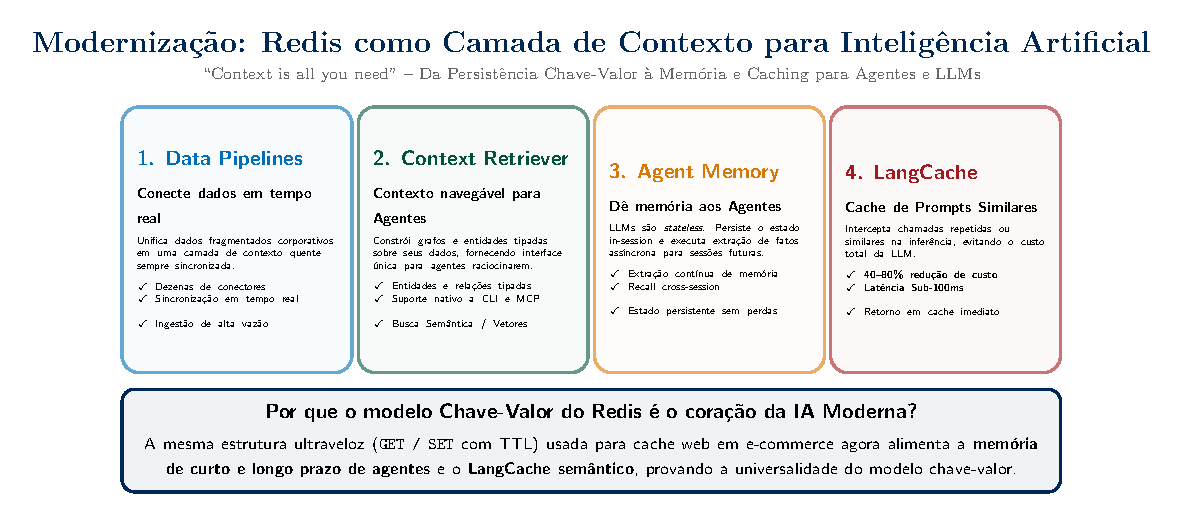
\includegraphics[width=0.90\textwidth,height=0.74\textheight,keepaspectratio]{figuras/fig_redis_ai_langcache.pdf}
\end{frame}

% ------------------------------------------------------------------------------
\twocolframe[title={Atividades Práticas e Próximos Passos},leftcol=7cm,rightcol=7cm]{%
  \alert{Laboratório Hands-On de Hoje}\par
  \itemseps[topsepi=2mm,itemsepi=3mm,labelsep=2mm,leftmargini=4mm]
  \begin{itemize}
    \item Executar o script de terminal \texttt{redis\_cli\_guia\_pratico.sh}.
    \item Praticar no terminal \texttt{redis-cli} as variações de \texttt{SET} (\texttt{NX}, \texttt{EX}, \texttt{KEEPTTL}) e \texttt{GET} (\texttt{GETDEL}, \texttt{MGET}).
    \item Testar a persistência disparando \texttt{BGSAVE} e inspecionando \texttt{LASTSAVE}.
    \item Rodar o script Python interativo \texttt{demonstracao\_aula04.py} e inspecionar os tempos de latência.
  \end{itemize}
}{%
  \alert{Conexão com a Aula 05}\par
  \itemseps[topsepi=2mm,itemsepi=3mm,labelsep=2mm,leftmargini=4mm]
  \begin{itemize}
    \item Na próxima aula (\textbf{Aula 05 - 20/10/2026}), aprofundaremos as \textbf{Estratégias Avançadas de Caching, Controle de Sessões e Filas de Mensagens (Streams)}.
    \item Resolver a lista de exercícios práticos da Aula 04 disponível no portal web da disciplina.
    \item O código e slides estão disponíveis no repositório oficial da turma.
  \end{itemize}
}
